\documentclass[a4paper,12pt]{book}
\usepackage[utf8]{inputenc}

%maths
\usepackage{amsmath}
\usepackage{amssymb}
\usepackage{amsthm}


%graphics
\usepackage{tikz}
\usetikzlibrary{fit,positioning}
\usetikzlibrary{arrows}

%algorithms
\usepackage{algorithm}
\usepackage{algorithmic}
\usepackage{caption}

%citations
\usepackage{natbib}

%hyperlinks
\usepackage{url}

%references
\usepackage{cleveref}

%others
\usepackage{enumerate}
\usepackage{breakcites}
\usepackage{nicefrac}

%box definition
\usepackage{tcolorbox}
\definecolor{mycolor}{rgb}{0.122, 0.435, 0.698}
\newtcbox{\mybox}{nobeforeafter,colframe=mycolor,colback=mycolor!10!white,boxrule=0.5pt,arc=4pt,
  boxsep=0pt,left=6pt,right=6pt,top=6pt,bottom=6pt,tcbox raise base}

%some definitions of symbols

\let\bb\mathbb       % BlackBoardBold (double letters)

  \def\AA{{\bb A}}\def\CC{{\bb C}}\def\DD{{\bb D}}\def\Ex{{\bb E}}
  \def\GG{{\bb G}}\def\HH{{\bb H}}\def\KK{{\bb K}}\def\LL{{\bb L}}
  \def\MM{{\bb M}}\def\QQ{{\bb Q}}\def\TT{{\bb T}}\def\YY{{\bb Y}}
  \def\PP{{\bb P}}\def\II{{\bb I}}\def\WW{{\bb W}}\def\XX{{\bb X}}
  \def\VV{{\bb V}}\def\SS{{\bb S}}\def\BB{{\bb B}}\def\NN{{\bb N}}
  \def\RR{{\bb R}}\def\ZZ{{\bb Z}}\def\FF{{\bb F}}\def\DD{{\bb D}}
  \def\OO{{\bb O}}\def\JJ{{\bb J}}\def\UU{{\bb U}}

\def\Ex{\mathbf E}
\def\calA{\mathcal A}
\def\calC{\mathcal C}
\def\calD{\mathcal D}
\def\calE{\mathcal E}
\def\calF{\mathcal F}
\def\calG{\mathcal G}
\def\calH{\mathcal H}
\def\calR{\mathcal R}
\def\calX{\mathcal X}
\def\calY{\mathcal Y}
\def\calV{\mathcal V}
\def\bb{\mathbb}
\def\hat{\widehat}
\def\bfX{\mathbf X}
\def\bfB{\mathbf B}
\def\bfA{\mathbf A}
\def\bfH{\mathbf H}
\def\bSigma{\boldsymbol\Sigma}
\def\bsigma{\boldsymbol\sigma}
\def\bOmega{\boldsymbol\Omega}
\def\beps{\boldsymbol\epsilon}
\def\bmu{\boldsymbol\mu}
\def\bnu{\boldsymbol\nu}
\def\btau{\boldsymbol\tau}
\def\bTau{\boldsymbol{\mathcal T}}
\def\btheta{{\boldsymbol\theta}}
\def\bTheta{{\boldsymbol\Theta}}
\def\bPi{\boldsymbol\Pi}
\def\bX{\boldsymbol X}
\def\bchi{\boldsymbol \chi}
\def\bA{\boldsymbol A}
\def\bF{\boldsymbol F}
\def\bx{\boldsymbol x}
\def\bu{\boldsymbol u}
\def\bv{\boldsymbol v}
\def\bS{\boldsymbol S}
\def\bbeta{\boldsymbol \beta}
\def\bY{\boldsymbol Y}
\def\bxi{\boldsymbol \xi}
\def\bpi{\boldsymbol \pi}
\def\bomega{\boldsymbol \omega}
\def\ci{\perp\!\!\!\perp}
\def\bZ{\boldsymbol Z}
\def\11{\mathds 1}
\def\b1{\mathbf 1}
\def\Pb{\mathbf P}
\def\var{{\bf Var}}
\def\KL{{\rm KL}}
\def\bfZ{\mathbf Z}
\def\bfI{\mathbf I}

\DeclareMathOperator*{\argmax}{arg\,max}
\DeclareMathOperator*{\argmin}{arg\,min}
\newcommand*{\pd}[3][]{\ensuremath{\frac{d^{#1} #2}{d#3^{#1}}}}

%definitions
\newtheorem{remark}{Remark}
\newtheorem{defi}{Definition}
\newtheorem{lem}{Lemma}
\newtheorem{cor}{Corollary}[section]
\newtheorem{pro}{Proposition}
\newtheorem{proposition}{Proposition}
\newtheorem{fact}{Fact}
\newtheorem{hyp}{Hypothesis}
\newtheorem{lemma}{Lemma}[section]
\newtheorem{prop}{Proposition}[section]
\newtheorem{theorem}{Theorem}[section]

\begin{document}

\author{Mehdi Sebbar}
\title{Thesis}
\date{2017}

\frontmatter
\maketitle
\tableofcontents

\mainmatter 
%!TEX root = ../main.tex

\chapter{Introduction}

The broad goal of this thesis is to tackle a clustering problem in the scope of mixtures model framework. More precisely, we will study the clustering of points drawn from high-dimensional Gaussian mixtures distributions. Thus, in the first part of this section we present the Gaussian mixture model and the second part we describe the well know  Expectation-Maximization algorithm (EM). We will also present the limitations of this algorithm in high-dimensional setting.

\section{The Gaussian mixture model}

The Gaussian mixture model is an important framework for clustering problems. It assumes that the observations are drawn from a
mixture distribution the components of which are Gaussian  with parameters $(\bmu_k,\bSigma_k)$:
\begin{equation}
\varphi_{\bmu_k,\bSigma_k}(x)=\frac{1}{(2\pi)^{p/2}|\bSigma_k|^{1/2}} \exp\Big(-\frac{1}{2}(\bx-\bmu_k)^\top\bSigma_k^{-1}(\bx-\bmu_k)\Big)
\end{equation}

Let $\btheta$ be the list containing all the unknown parameters of a Gaussian mixture model: the family of means $\bmu = (\bmu_1,\ldots,\bmu_K)
\in (\RR^p)^K$, the family of covariance matrices $\bSigma = (\bSigma_1,\ldots,\bSigma_k)\in(\mathcal S_{++}^p)^K$ and the vector of cluster probabilities  $\bpi=(\pi_1,\ldots,\pi_k)\in [0,1]^K$ such that $\b1_p^\top\bpi=1$.
The density of one observation $\bX_1$ is then given by:
\begin{equation}\label{mixture}
p_{\btheta}(\bx)=\sum_{k=1}^K\pi_k\varphi_{\bmu_k,\bSigma_k}(\bx),\qquad \forall \bx\in\RR^p,
\end{equation}
where $\btheta=(\bmu,\bSigma,\bpi)$.


This model can be interpreted from a latent variable perspective. Let $Z$ be a discrete random variable
taking its values in the set $[K]$ and such that $\Pb(Z=k) = \pi_k$ for every $k\in[K]$. The random variable $Z$
indicates the cluster from which the observation $\bX$ is drawn.  Considering that all the conditional distributions
$\bX|Z=k$ are Gaussian, we get the following formula for the marginal density of $X$:
\begin{equation}
p_{\btheta}(\bx)=\sum_{k=1}^K \Pb(Z=k)p_{\theta}(\bx|Z=k) = \sum_{k=1}^K\pi_k\varphi_{\bmu_k,\bSigma_k}(\bx),\qquad \forall \bx\in\RR^p.
\end{equation}
In the clustering problem, the goal is to assign $X$ to a cluster or, equivalently, to predict the cluster $Z$ of the vector $\bX$.
A prediction function in such a context is $g:\RR^p\to[K]$ such that $g(\bX)$ is as close as possible to $Z$. If we measure the
risk of a prediction function $g$ in terms of misclassification error rate $R_\btheta(g) = \Pb_\btheta(g(\bX)\not=Z)$, then it is
well known that the optimal (Bayes) predictor $g^*_\btheta \in \arg\min_g R_\btheta(g)$ is provided by the rule
$$
g^*_\btheta(\bx) = \arg\max_{k\in [K]} \tau_k(\bx,\btheta),
$$
where $\tau_k(\bx,\btheta)=p_{\btheta}(Z=k|\bX=\bx)$ stands for the conditional probability of the latent variable $Z$ given $\bX$.
In the Gaussian mixture model, Bayes's rule implies that
\begin{equation}
\label{tau_bayes}
\tau_k(\bx,\btheta)=\frac{p_{\btheta}(\bx|Z=k)\Pb(Z=k)}{p_{\btheta}(\bx)}
=\frac{\pi_k\varphi_{\bmu_k,\bSigma_k}(\bx)}{\sum_{k'=1}^K\pi_{k'}\varphi_{\bmu_{k'},\bSigma_{k'}}(\bx)}
\end{equation}


Since the true value of the parameter $\btheta$ is not available, formula (\ref{tau_bayes}) can not be
directly used for solving the problem of clustering. Instead, a natural strategy is to estimate $\btheta$
by some vector $\hat\btheta$, based on a sample $\bX_1,\ldots,\bX_n$ drawn from the density $p_\btheta$, and
then to define the clustering rule by
\begin{equation}
\label{gen_clust}
\hat g(\bx) = g^*_{\hat\btheta}(\bx)=\arg\max_{k\in [K]} \tau_k(\bx,\hat\btheta)=\arg\max_{k\in [K]}\
\hat\pi_k\varphi_{\hat\bmu_k,\hat\bSigma_k}(\bx).
\end{equation}
A common approach to estimating the parameter $\btheta$ is to rely on the likelihood maximization.

Let $\bX_1,\dots,\bX_n$ with $\bX_i\in \RR^p$ be a set of iid observations drawn from the density $p_{\btheta}$
given by (\ref{mixture}). The following graphical model depicts the scheme of the observations:
%%GRAPH of pgm
\begin{figure}[h]
\centering\small
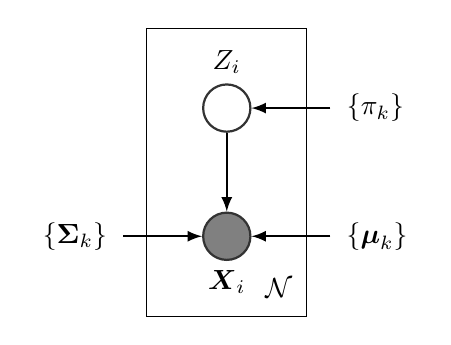
\begin{tikzpicture}
\tikzstyle{main}=[circle, minimum size = 6mm, thick, draw =black!80, node distance = 10mm]

\tikzstyle{connect}=[-latex, thick]
\tikzstyle{box}=[rectangle, draw=black!100]
  \node[main, fill = black!50] (x) [label=below:{$\bX_i$}] { };
  \node[main] (z) [above=of x,label=above:{$Z_i$}] {};

  \path (z) edge [connect] (x);

  \node[rectangle, inner sep=7mm,draw=black!100, fit= (z) (x)] {};
\node[rectangle, below=of x, inner sep=-10mm, fit= (z) (x),label=below right:{$\!\mathcal N$}, xshift=4mm,yshift=-2mm] {};

\node[main,draw=none] (a) [right=of x] {$\{\bmu_k\}$};
\path (a) edge [connect] (x);
\node[main,draw=none] (b) [left=of x] {$\{\bSigma_k\}$};
\path (b) edge [connect] (x);
\node[main,draw=none] (c) [right=of z] {$\{\pi_k\}$};
\path (c) edge [connect] (z);
\end{tikzpicture}
\end{figure}

The log-likelihood of the Gaussian mixture model is
\begin{equation}\label{log-likelihood}
\ell_n(\btheta)=\sum_{i=1}^{n}\log{p_{\btheta}(\bx_i)}=
\sum_{i=1}^{n}\log\bigg\{{\sum_{k=1}^K\pi_k\varphi_{(\bmu_{k},\bSigma_{k})}(\bx_i)}\bigg\}.
\end{equation}
Because of the presence in this equation of the logarithm of a sum, the maximization of the log-likelihood is
a difficult nonlinear and nonconvex problem. In particular, this is not a exponential family distribution yielding simple expressions.
A commonly used approach for approximately maximizing (\ref{log-likelihood}) with respect to $\btheta$ is the Expectation-Maximization
(EM) Algorithm \citep{dempster77} that we recall below.

Summarizing the content of this section, we can describe the following  natural approach to solving the clustering problem under Gaussian
mixture modeling assumption:
\begin{figure}[H]
\begin{center}
\mybox{
\begin{minipage}{0.85\linewidth}
\begin{algorithmic}%[1]\tt
\small
\STATE {\bfseries Input:} data vectors $\bx_1,\ldots,\bx_n\in\RR^p$ and the number of clusters $K$
\STATE {\bfseries Output:} function  $\hat g : \RR^p\to [K]$
\STATE {\tt 1: Estimate $\btheta=(\bpi,\bmu,\bSigma)$ by maximizing the log-likelihood:}
\begin{align}\label{step:1}
\hat\btheta
    &\in\arg\max_{\btheta\in\bTheta}  \ell(\btheta|\bx_1,\dots,\bx_n)
    =\arg\max_{\bpi,\bmu,\bSigma}  \sum_{i=1}^{n}\log\bigg\{{\sum_{k=1}^K\pi_k\varphi_{\bmu_{k},\bSigma_{k}}(\bx_i)}\bigg\}.
\end{align}
\STATE {\tt 2: Output the clustering rule:}
\begin{equation}
\label{step:2}
\hat g(\cdot) = \arg\max_{k\in [K]} \hat\pi_k\varphi_{\hat\bmu_k,\hat\bSigma_k}(\cdot).
\end{equation}
\end{algorithmic}
\end{minipage}
}
   \caption{Clustering under Gaussian mixture modeling}
   \label{algo:general}
\end{center}
\vspace{-15pt}
\end{figure}


\section{EM Algorithm}

The goal of the EM algorithm is to approximate a solution of the problem \eqref{step:1}.
Since this optimization problem contains a nonconvex cost function, it is impossible to
design a polynomial time algorithm that provably converges to the global maximum point. Instead,
the EM algorithm provides a sequence $\{\hat\btheta(t)\}_{t\in\NN}$ of parameter values such that
the cost function (\textit{i.e.}, the log-likelihood) evaluated at these values forms an
increasing sequence that converges to a local maximum.

The main idea underlying the EM algorithm is the following representation of the log-likelihood
of one observation derived from the log-sum inequality:
\begin{equation}\label{hint}
\log\bigg\{{\sum_{k=1}^K\pi_k\varphi_{\bmu_{k},\bSigma_{k}}(\bx_i)}\bigg\} =
\max_{\substack{\btau\in[0,1]^K \ \btau^\top \b1_K=1}} \sum_{k=1}^K \Big\{\tau_{k}\log\varphi_{\bmu_{k},\bSigma_{k}}(\bx_i)+\tau_{k} \log(\pi_k/\tau_{k})\Big\}.
\end{equation}
Let us denote by $\bTau = (\tau_{i,k})$ a $n\times K$ matrix with nonnegative entries such that $\bTau\b1_K = \b1_n$, that is each
row of $\bTau$ is a probability distribution on $[K]$. Combining \eqref{step:1} and \eqref{hint}, we get
\begin{align}\label{eq:3}
\hat\btheta
    &\in\argmax_{\btheta=(\bpi,\bmu,\bSigma)}\max_{\bTau}
    \sum_{i=1}^{N} \sum_{k=1}^K \Big\{\tau_{i,k}\log\varphi_{\bmu_{k},\bSigma_{k}}(\bx_i)+\tau_{i,k}
    \log(\pi_k/\tau_{i,k})\Big\}.
\end{align}
The great advantage of this new representation of the log-likelihood function is that the cost
function in \eqref{eq:3}, considered as a function of $\btheta$ and $\bTau$, is biconcave, \textit{i.e.},
it is concave with respect to $\btheta$ for every fixed $\bTau$ and concave with respect to $\bTau$ for
every fixed $\btheta$. In such a situation, one can apply the alternating maximization approach to sequentially
improve on an initial point. In the present context, an additional attractive feature of the cost function
in \eqref{eq:3} is that the two optimization problems involved in the alternating maximization procedure
admit explicit solutions.

\begin{figure}[ht]
\begin{center}
\mybox{
\begin{minipage}{0.85\linewidth}
\begin{algorithmic}%[1]\tt
%\SetLine%\SetAlgoLined
\small
\STATE {\bfseries Input:} data vectors $\bx_1,\ldots,\bx_n\in\RR^p$ and the number of clusters $K$
\STATE {\bfseries Output:} parameter estimate $\hat\btheta = \{\hat\bmu_k,\hat\bSigma_k,\pi_k\}_{k\in[K]}$
\STATE {\tt 1: Initialize $t=0$, $\btheta=\btheta^0$.}
\STATE {\tt 2: {\bf Repeat}}
\STATE \qquad {\tt 3: Update the parameter $\bTau$:}
\begin{align*}
\tau_{i,k}^{t}  &= \frac{\pi_k^{t}\varphi_{\bmu_k^{t},\bSigma_k^{t}}(\bx_i)}{\sum_{k'\in[K]}\pi^{t}_{k'}\varphi_{\bmu^{t}_{k'},\bSigma^{t}_{k'}}(\bx_i)}.
\end{align*}
\STATE \qquad{\tt 4: Update the parameter $\btheta$:}
\begin{align*}
\pi_k^{t+1}     &= \frac1n\sum_{i=1}^n \tau_{i,k}^t,\qquad
\bmu_k^{t+1}    = \frac1{n\pi_k^{t+1}}\sum_{i=1}^n \tau_{i,k}^t\bx_i,\\
\bSigma_k^{t+1} &= \frac1{n\pi_k^{t+1}}\sum_{i=1}^n \tau_{i,k}^t(\bx_i-\bmu_k^{t+1})(\bx_i-\bmu_k^{t+1})^\top.
\end{align*}
\STATE \qquad {\tt 5: increment $t$: $t=t+1$}.
\STATE {\tt 6: {\bf Until} stopping rule.}
\STATE {\tt 7: {\bf Return} $\btheta^{t}$}.
\end{algorithmic}
\end{minipage}}
   \caption{EM algorithm for Gaussian mixtures}
   \label{algo:EM}
\end{center}
\end{figure}


\begin{lem}
\label{lemma1}
Let us introduce the cost function
\begin{equation}
F(\btheta,\bTau) = \sum_{i=1}^{n} \sum_{k=1}^K \Big\{\tau_{i,k}\log\varphi_{\bmu_{k},\bSigma_{k}}(\bx_i)+\tau_{i,k}
    \log(\pi_k/\tau_{i,k})\Big\}.
\end{equation}
Then, the following two optimization problems
\begin{align}
\hat\btheta(\bTau)&\in \arg\max_{\btheta} F(\btheta,\bTau),\qquad \hat\bTau(\btheta)\in \arg\max_{\bTau} F(\btheta,\bTau)
\end{align}
has explicit solutions given by
\begin{align}
\label{em-sols}
\hat\pi_k     &= \frac1n\sum_{i=1}^n \tau_{i,k},\qquad\hat\bmu_k = \frac1{n\hat\pi_k}\sum_{i=1}^n \tau_{i,k}\bx_i ,\qquad \forall k\in[K],\\
\hat\bSigma_k &= \frac1{n\hat\pi_k}\sum_{i=1}^n \tau_{i,k}(\bx_i-\hat\bmu_k)(\bx_i-\hat\bmu_k)^\top,\qquad\forall k\in[K],\\
\hat\tau_{i,k}&= \frac{\pi_k\varphi_{\bmu_k,\bSigma_k}(\bx_i)}{\sum_{k'\in[K]}\pi_{k'}\varphi_{\bmu_{k'},\bSigma_{k'}}(\bx_i)},\qquad\forall k\in[K],\ \forall i\in[n].
\end{align}
\end{lem}

Based on this result, the EM algorithm is defined as in Figure~\ref{algo:EM}.
The algorithm operates iteratively and needs a criterion to determine when
the iterations should be stopped. There is no clear consensus on this point in the
statistical literature, but it is a commonly used  practice to stop when one of the
following conditions is fulfilled:
\begin{description}
\item[i)]  The number of iterations $t$ exceeds a pre-specified level $t_{\max}$.
\item[ii)] The increase of the log-likelihood over past $t_0$ iterations is not
significantly different from zero: $\ell_n(\btheta^{t})-\ell_n(\btheta^{t-t_0})\le \varepsilon$
for some pre-specified values $t_0\in\NN$ and $\varepsilon>0$.
\end{description}
EM is conceptually easy and each iteration increases the log-likelihood:
$$
\ell_n(\btheta^{t+1})\ge \ell_n(\btheta^{t}),\qquad \forall t\in\NN.
$$
The complexity at each step of the EM algorithm is $O(Knp^2)$ and
it usually requires many iterations to converge. In a high-dimensional setting
when $p$ is large, the quadratic dependence on $p$ may result in prohibitively
large running times. However, the computation of the elements of the covariance
matrices $\bSigma^t_k$ and the mean vectors $\bmu^t_k$ can be parallelized which
may lead to considerable savings in the running time.

\include{./TeX_files/Graphical_Lasso_for_Gaussian_mixtures}
%!TEX root = ../main.tex

\chapter{Estimating the number of clusters}

The idea is to add a regularization term on the estimation of the $n\times K$ matrix $\bTau$, the estimate of the number of clusters K will be the number of non-empty columns of $\bTau$.\

We consider a maximum number of clusters $M$, we note the convex set $A=\{\tau \in \RR^M : \sum_{k=1}^M\tau_k=1, \tau_k\geq 0 \quad \forall k \in [M] \}$ and the "indicator" function $\chi_A(.)$ defined by:


  \begin{equation*}
    \chi_A(x) =
    \begin{cases}
      0 & \text{if } x \in A,\\
      	\infty & \text{if } x = 0
    \end{cases}
\end{equation*}

We note $\bTau_{.,k}$ the $k^{th}$ column and $\bTau_{i,.}$ the $i^{th}$ line of $\bTau$. We will estimate $\bTau$ using the same equation \ref{cost_fun_pen}, \ref{optim-problems} with a regularization term:\\
\begin{align*}
F^{pen}(\btheta,\bTau)  =& \sum_{k=1}^K \bigg(\sum_{i=1}^{n} \Big\{\tau_{i,k}\log\varphi_{\bmu_{k},\bOmega_{k}}(\bx_i)+\tau_{i,k}
    \log(\pi_k/\tau_{i,k})\Big\}-\lambda_k||\bOmega_k||_{1,1}\bigg)\\ 
    &+ \sum_{k=1}^K ||\bTau_{.,k}||_{2} + \sum_{i=1}^{n} \chi_A(\bTau_{i,.})
\end{align*}
Removing the penalization on $\bOmega$:

\begin{align*}
F^{pen}(\btheta,\bTau)  =& \sum_{k=1}^K \bigg(\sum_{i=1}^{n} \Big\{\tau_{i,k}\log\varphi_{\bmu_{k},\bOmega_{k}}(\bx_i)+\tau_{i,k}
    \log(\pi_k/\tau_{i,k})\Big\}\\ 
    &+ \sum_{k=1}^K ||\bTau_{.,k}||_{2} + \sum_{i=1}^{n} \chi_A(\bTau_{i,.})
\end{align*}

 and the optimization problem:
\begin{equation}
\hat\bTau(\btheta)\in \arg\max_{\bTau} F^{pen}(\btheta,\bTau)
\end{equation}

Unfortunately, the regularization term prevents to derive explicit solution as in previous chapters. Furthermore, we cant separate the objective function since we optimize along columns and lines of $\bTau$. The objective function $F^{pen}(\btheta,\bTau)$ rewritten
$F^{pen}_{\btheta}(\bTau)$ can be split into two terms:

\begin{equation}
F^{pen}_{\btheta}(\bTau)={\large f}({\footnotesize
\bTau})+ {\large g}({\footnotesize
\bTau})
\end{equation}

with:

\begin{align*}
f(\bTau) =& 	\sum_{k=1}^K \bigg(\sum_{i=1}^{n} \Big\{\tau_{i,k}\log\varphi_{\bmu_{k},\bOmega_{k}}(\bx_i)+\tau_{i,k} \log(\pi_k/\tau_{i,k})\Big\} + \sum_{k=1}^K ||\bTau_{.,k}||_{2}\\
g(\bTau) =& \sum_{i=1}^{n} \chi_A(\bTau_{i,.})
\end{align*}

$f$ is convex and differentiable on its domain, $g$ is also convex but not smooth. We will tackle this problem by using a proximal method:

\begin{align*}
	\bTau^{k+1} =& {\bf{prox}}_{\lambda g}(\bTau^k - \lambda \nabla f(\bTau^k))\
			=& P_A(\bTau^k - \lambda \nabla f(\bTau^k))\\
			=&\argmin_{ \bTau : \forall K, \bTau^k \in A}\big( || \bTau - (\bTau^k - \lambda \nabla f(\bTau^k) ) ||^2_2 \big)
\end{align*}

The gradient of f on $\bTau$ is given by:

\begin{align*}
\bigg[\nabla_{\bTau}f(\bTau)\bigg]_{i,j} =& \bigg[\frac{\partial f}{\partial \bTau_{ij}}(\bTau) \bigg]_{i,j}\\
=& \log(\varphi_{\bmu_j,\bOmega_j}(x_i))+\log(\frac{\pi_j}{\tau_{i,j}})+\frac{\tau_{i,j}}{||\bTau_{.,j}||_2}-1
\end{align*}

We will use FISTA to accelerate the convergence

\begin{figure}
\begin{center}
\mybox{
\begin{minipage}{0.85\linewidth}
\begin{algorithmic}%\SetAlgoLined\tt\SetLine
\small
\STATE {\bfseries Input:} 
\STATE {\bfseries Output:} parameter estimate $\bTau$
\STATE {\tt 1: Initialize $t_1=1$ and $\bxi^0$ with}
\begin{align*}
\xi_{i,k}^{0}  &= \frac{\pi_k^{0}\varphi_{\bmu_k^{0},\bOmega_k^{0}}(\bx_i)}{\sum_{k'\in[K]}\pi^{0}_{k'}\varphi_{\bmu^{0}_{k'},\bOmega^{0}_{k'}}(\bx_i)}
\end{align*}
\STATE {\tt 2: {\bf Repeat}}
\begin{align*}
\bTau^k =&\argmin_{ \bTau : \forall K, \bTau^k \in A}\big( || \bTau - (\bxi^k - \lambda \nabla f(\bxi^k) ) ||^2_2 \big)\\
t^{k+1} =& \frac{1+\sqrt{1+4*(t^k)^2}}{2}\\
\bxi^{k+1} =& \bTau^k + \bigg( \frac{t^k-1}{t^{k+1}}\bigg) \big( \bTau^k - \bTau^{k-1} \big)
\end{align*}
\end{algorithmic}
\end{minipage}}
   \caption{ $\bTau$ estimation with FISTA}
   \label{algo:PEM}
\end{center}
\end{figure}

We use the algorithm of last chapter with the new estimation procedure of $\bTau$ 

\begin{figure}
\begin{center}
\mybox{
\begin{minipage}{0.85\linewidth}
\begin{algorithmic}%\SetAlgoLined\tt\SetLine
\small
\STATE {\bfseries Input:} data vectors $\bx_1,\ldots,\bx_n\in\RR^p$ and the number of clusters $K$
\STATE {\bfseries Output:} parameter estimate $\hat\btheta = \{\hat\bmu_k,\hat\bOmega_k,\hat\pi_k\}_{k\in[K]}$
\STATE {\tt 1: Initialize $t=0$, $\btheta=\btheta^0$.}
\STATE {\tt 2: {\bf Repeat}}
\STATE {\tt 3: \qquad Update the parameter $\bTau$ with previous algorithm}
\STATE {\tt 4: \qquad Update the parameter $\btheta$:}
\begin{align*}
\pi_k^{t+1}     &= \frac1n\sum_{i=1}^n \tau_{i,k}^t,\qquad \\
\bmu_k^{t+1}    &= \frac1{n\pi_k^{t+1}}\sum_{i=1}^n \tau_{i,k}^t\bx_i\\
\bSigma_{n,k}         &= \frac{1}{n^2\pi_k^{t+1}}\sum_{i=1}^n\tau_{i,k}^{t+1}(\bx_i-\hat\bmu_k^{t+1})(\bx_i-\hat\bmu_k^{t+1})^\top\\
\bOmega_k^{t+1} & \in \argmin_{ \bOmega\succeq 0} \Big\{ -\frac{1}{2}\log| \bOmega |+\frac{1}{2} tr(\bSigma_{N,k}\bOmega)+\frac{\lambda_k}{n\pi_k^{t+1}}||\bOmega||_{1,1}\Big\}
\end{align*}
\STATE {\tt 5: \qquad increment $t$: $t=t+1$}.
\STATE {\tt 6: {\bf Until} stopping rule.}
\STATE {\tt 7: {\bf Return} $\btheta^{t}$}.
\end{algorithmic}
\end{minipage}}
   \caption{Graphical lasso algorithm for Gaussian mixtures with cluster number discovery}
   \label{algo:PEM}
\end{center}
\end{figure}

\include{./TeX_files/algorithm2}
\include{./TeX_files/lasso}
\include{./TeX_files/chapter02}
%!TEX root = ../main.tex

\chapter{Numerical Experiments}

In this section we describe the implementation of the algorithm. We also compare its performance with different alternative methods.

\subsection{Implementation details}

The implementation of this algorithm is straight forward

\subsection{Alternative methods}
\subsubsection{SPADES}
From \cite{SPADES}
\subsection{Adaptive Dantzig density estimation}
From \cite{Bertin}
\subsubsection{kernel density estimation}

\subsection{Experimental Evaluations}

\backmatter
% bibliography, glossary and index would go here.

\bibliographystyle{plain}
\bibliography{ref}

\end{document}